\documentclass[tikz,border=5pt]{standalone}
\usepackage{amsmath}
\usetikzlibrary{arrows.meta,calc,decorations.pathreplacing}
\definecolor{ink}{HTML}{16324F}
\definecolor{teal}{HTML}{168A88}
\definecolor{gold}{HTML}{D9892B}
\definecolor{redq}{HTML}{B84A4A}
\definecolor{glass}{HTML}{D9E3EA}
\begin{document}
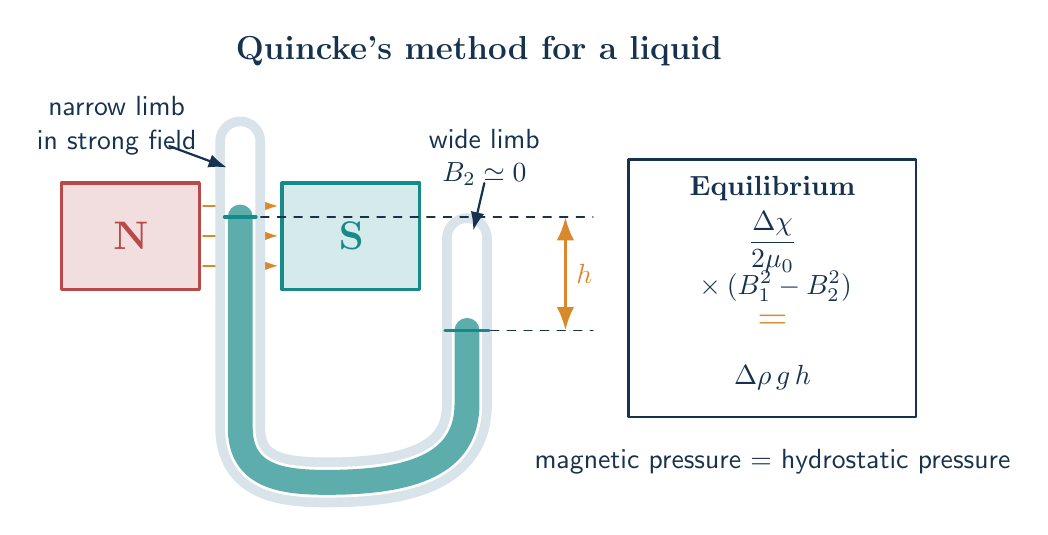
\begin{tikzpicture}[font=\sffamily,>=Latex,line cap=round,line join=round]
  \node[font=\bfseries\large,ink] at (5.65,5.72) {Quincke's method for a liquid};

  % Magnet pole pieces around the narrow limb
  \fill[redq!18] (.35,2.7) rectangle (2.1,4.05);
  \draw[redq,very thick] (.35,2.7) rectangle (2.1,4.05);
  \node[redq,font=\bfseries\Large] at (1.23,3.38) {N};
  \fill[teal!18] (3.15,2.7) rectangle (4.9,4.05);
  \draw[teal,very thick] (3.15,2.7) rectangle (4.9,4.05);
  \node[teal,font=\bfseries\Large] at (4.03,3.38) {S};
  \foreach \y in {3.0,3.38,3.76}
    \draw[->,gold,thick] (2.15,\y)--(3.1,\y);
  \node[gold] at (2.62,4.27) {$B_1$};

  % Glass U tube, then liquid inside
  \draw[glass,line width=18pt]
    (2.62,4.58)--(2.62,.95)
    .. controls (2.62,.32) and (3.15,.25) .. (3.72,.25)
    .. controls (4.8,.25) and (5.5,.48) .. (5.5,1.25)
    --(5.5,3.35);
  \draw[white,line width=11pt]
    (2.62,4.58)--(2.62,.95)
    .. controls (2.62,.32) and (3.15,.25) .. (3.72,.25)
    .. controls (4.8,.25) and (5.5,.48) .. (5.5,1.25)
    --(5.5,3.35);
  \draw[teal!70,line width=9pt]
    (2.62,3.62)--(2.62,.95)
    .. controls (2.62,.32) and (3.15,.25) .. (3.72,.25)
    .. controls (4.8,.25) and (5.5,.48) .. (5.5,1.25)
    --(5.5,2.18);
  \draw[teal,very thick] (2.42,3.62)--(2.82,3.62);
  \draw[teal,very thick] (5.22,2.18)--(5.78,2.18);

  % Hydrostatic head
  \draw[ink,dashed] (2.88,3.62)--(7.1,3.62);
  \draw[ink,dashed] (5.8,2.18)--(7.1,2.18);
  \draw[<->,gold,very thick] (6.75,2.18)--(6.75,3.62) node[midway,right] {$h$};
  \node[ink,align=center] at (1.05,4.78) {narrow limb\\in strong field};
  \draw[->,ink,thick] (1.72,4.52)--(2.45,4.25);
  \node[ink,align=center] at (5.72,4.38) {wide limb\\\(B_2\simeq0\)};
  \draw[->,ink,thick] (5.72,4.05)--(5.58,3.45);

  % Measurement and balance statement
  \draw[ink,thick] (7.55,1.08) rectangle (11.2,4.35);
  \node[ink,font=\bfseries] at (9.38,3.98) {Equilibrium};
  \node[ink,align=center] at (9.38,3.12)
    {$\displaystyle \frac{\Delta\chi}{2\mu_0}$\\[-2pt]
     \(\displaystyle {}\times(B_1^2-B_2^2)\)};
  \node[gold,font=\bfseries\Large] at (9.38,2.28) {$=$};
  \node[ink] at (9.38,1.58) {$\Delta\rho\,g\,h$};
  \node[ink,align=center] at (9.38,.52)
    {magnetic pressure \(=\) hydrostatic pressure};
\end{tikzpicture}
\end{document}
